\section{Snorken}\label{section:snorken}
Snorken er en åbenlys faktor, der skal tages højde for når man skal opdage søvn ved hjælp af sensorer, idet en af de primære sensorer, som bruges til at bestemme om en person sover er lyd.
Den efterfølgende beskrevne proof of concept løsning håndterer ikke snorken, men overvejelser vi har haft om snorken nævnes her, og er strategier vi er klar over kan bruges med videre arbejde.

Et eksempel kan ses i \cref{fig:snorke-vs-ikkesnorken} hvor vi sammenligner en person som vi ved snorker mod en som ikke snorker.

\begin{figure}[h]
\begin{subfigure}{0.49\textwidth}
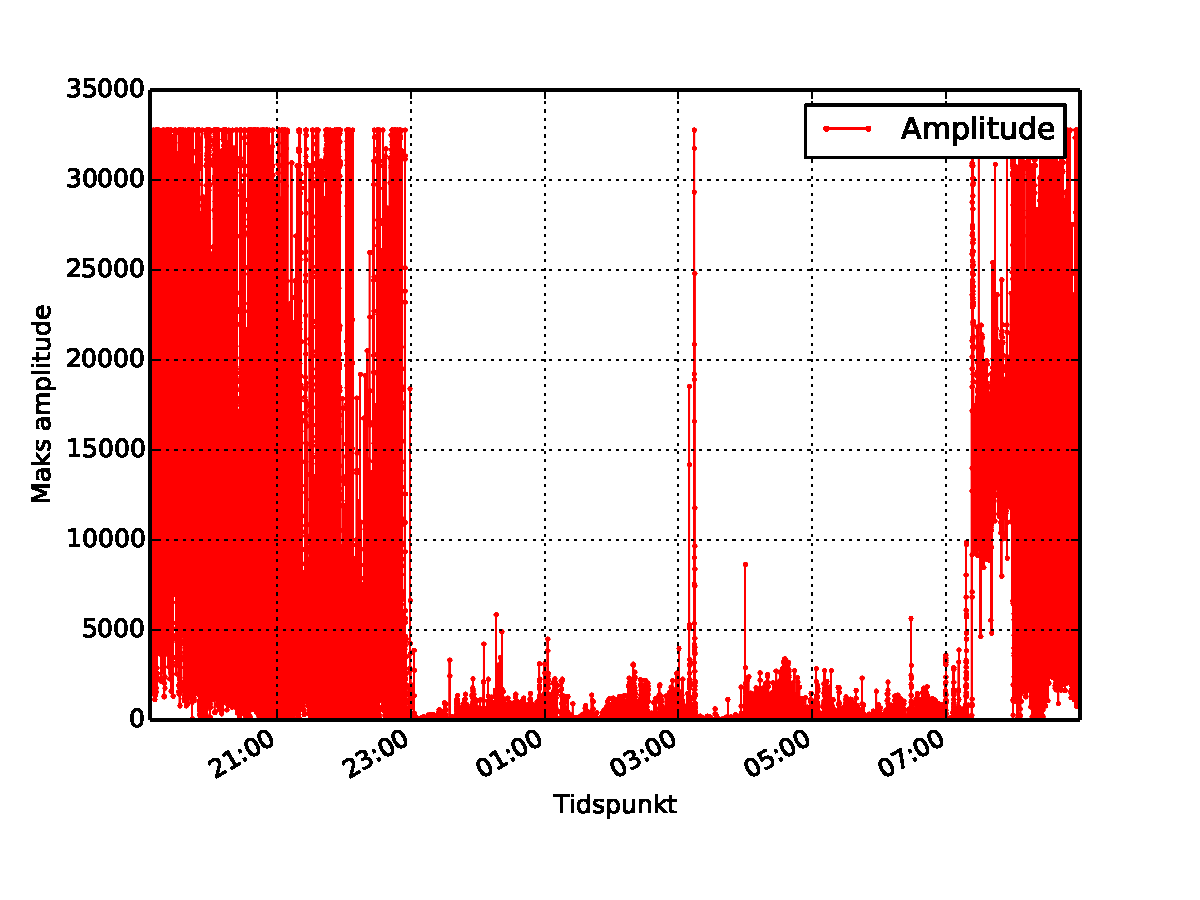
\includegraphics[width=1\textwidth,trim = 0cm 1cm 1cm 1cm,clip]{amplitude-plot-snorken}
\caption{Person der snorker}
\label{fig:person-snorker}
\end{subfigure}
\begin{subfigure}{0.49\textwidth}
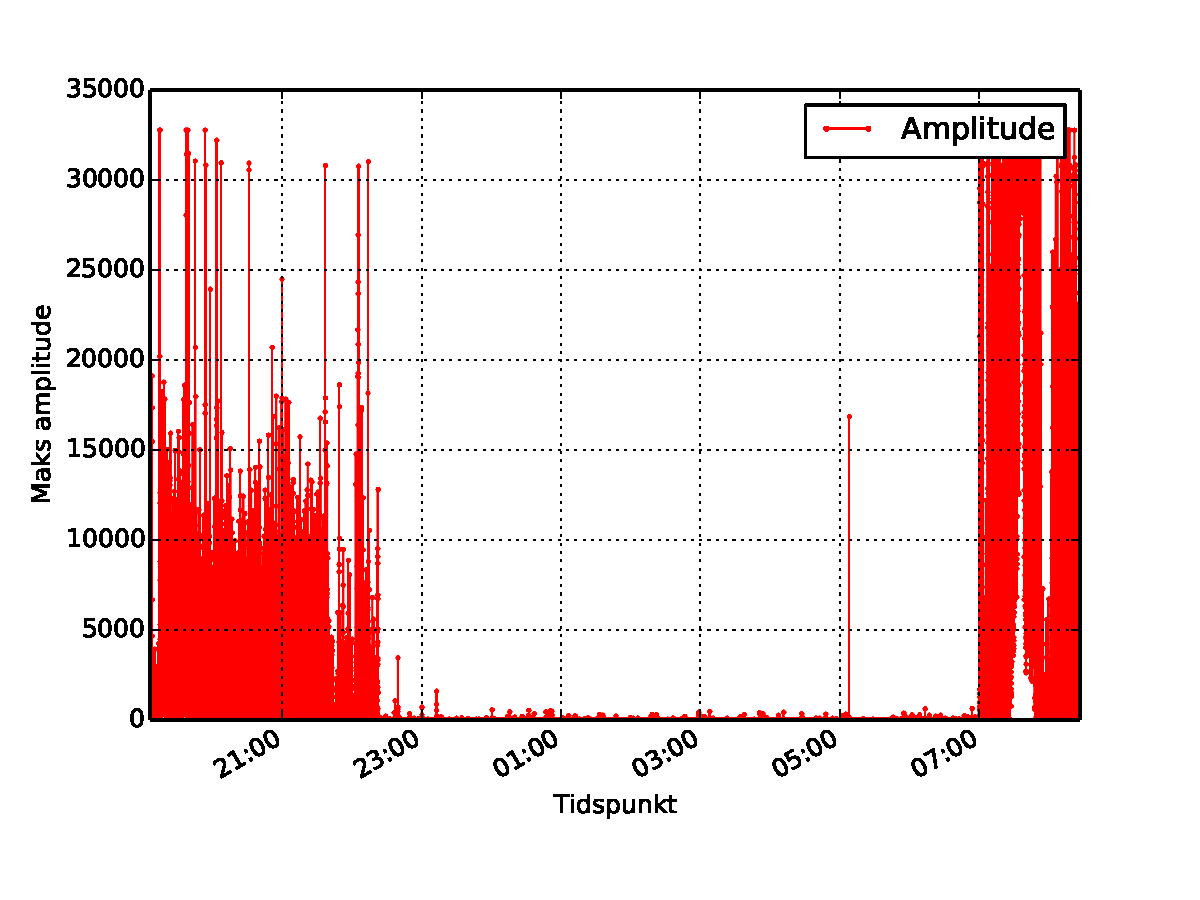
\includegraphics[width=1\textwidth,trim = 0cm 1cm 1cm 1cm,clip]{amplitude-plot-ingen-snorken}
\caption{Person der ikke snorker}
\label{fig:person-ikke-snorker}
\end{subfigure}
\caption{Person vi ved snorker og person vi ved ikke snorker}
\label{fig:snorke-vs-ikkesnorken}
\end{figure}

Hvis man ser på grafen med snorken, \cref{fig:person-snorker}, kan man se at amplituden er mere irregulær i søvnperioden i forhold til grafen i \cref{fig:person-ikke-snorker}.
En simpel løsning på hvordan man kunne ignorere snorken i en løsning, vil være at bruge en amplitude tærskelværdi, hvilket baseret på graferne kan være 5000. 
Tærskelværdien sætter grænsen for hvilken amplitude vi betragter som stilhed eller ej.
Men dette skal være baseret på hvor højt personen snorker og skal derfor være dynamisk, hvilket kan gøre at denne løsning ikke er optimal. 
Derudover, kan man ikke garantere at der ikke findes personer, der snorker lige så højt som når de snakker.
Andre metoder på at registrere søvn er derfor undersøgt.

Ud fra artiklerne \citet{Dafna2013}, \citet{Calabrese20111101} og \citet{7051338} dannes der et grundlag for hvordan snorken kan registreres.

\citet{Dafna2013} gør brug af et system til at inddele snorken og andre akustiske hændelser gennem et søvnforløb ved brug af lyd data, der blev optaget med en mikrofon ved en polisomnigrafisk undersøgelse. 
De endte med et meget præcist system, som kunne adskille snorken og andre akustiske hændelser med ~98\% nøjagtighed.

\citet{Calabrese20111101} foreslår et system, der skal bruges til diagnosticering af søvnapnø ved hjælp af optaget lyd.
Dog blev der kun implementeret en prototype af systemet og den er derfor ikke blevet evalueret ordenligt endnu. 
Idéen er at man bruger analyser såsom 'Fast Fourier Transform' og 'Power Spectrum' til at finde tidspunkter, hvor personen har snorket baseret på optaget lyd. 

\citet{7051338} udvikler et system, der kan registrer snorken ud fra lydoptagelser.
Denne metode bruger machine learning til at udvikle en model der detektere hvornår folk sover.
Metoden der er udviklet gør brug af en \textit{K}-Nearest Neighbour classifier.
I modsætning til \citet{Calabrese20111101}, fokuseres der på at registre snorken, hvilket også kvalificerer denne metode som en oplagt kandidat til videre udforskning.

Ved disse metoder benyttes lyd data og ikke bare amplituden, så det vil være nødvendigt at undersøge om systemet også kan fungere ved brug af amplitude.
Grunden til at vi bruger amplituden, er at alt data gemmes og intet slettes. 
Hvis løsningen ændres således at data analyseres løbende og slettes efterfølgende kan lyd data godt bruges, hvilket gør at vi undgår problemet med privatlivets fred.

De metoder betragtes relevante til at styrke ens model, da snorken er en tydelig indikator på at man sover, fremfor blot at blive betragtet som støj.
I den efterfølgende beskrevet proof of concept løsning er disse metoder dog ikke blevet benyttet, men kan med fordel betrages ved videre arbejde.